\documentclass{beamer}
\usepackage{appendixnumberbeamer}

\mode<presentation>{\usetheme[subsectionpage=progressbar,block=fill,numbering=none]{metropolis}}

\usepackage[english]{babel} 
\usepackage[utf8]{inputenc}

\usepackage{standalone}
\usetikzlibrary{calc,arrows.meta,positioning}
\usepackage{tikz-3dplot}
\usepackage{graphicx} % Allows including images
\usepackage{tikz}
\usepackage{pgfplots}
\pgfplotsset{compat=1.13}
\usepackage{pgfplotstable}
\usepackage{caption}
\usepackage{booktabs} % Allows the use of \toprule, \midrule and \bottomrule in tables
\usepackage{multicol} 

% Math packages
\usepackage{amsmath}
\usepackage{mathtools}
\usepackage{amssymb}
\usepackage{mathpartir}

% Coloured boxes
\usepackage{tcolorbox}
\colorlet{alert}{mLightBrown}
\newtcolorbox{alertbox}
{standard jigsaw, opacityback=0,colframe=alert}
\newtcolorbox{tbox}
{standard jigsaw, opacityback=0,opacityframe=0}

% Custom commands
\DeclarePairedDelimiter\ceil{\lceil}{\rceil}
\DeclarePairedDelimiter\floor{\lfloor}{\rfloor}
\DeclareMathOperator*{\argmin}{arg\,min}
\DeclareMathOperator*{\argmax}{arg\,max}
\newcommand{\mx}{\mathcal{X}}
\newcommand{\inp}{\mathcal{I}}
\newcommand{\costs}{c}
\newcommand{\opcosts}{c_{op}}
\newcommand{\swcosts}{c_{sw}}
\newcommand{\aswcosts}{\widehat{c}_{sw}}
\newcommand{\beps}{\boldsymbol\varepsilon}
\newcommand{\fromto}[2]{\{#1,\dotsc,#2\}}
\newcommand{\dotcup}{\mathbin{\mathaccent\cdot\cup}}

\title{Algorithms for Dynamic Right-Sizing in\\Data Centers} % The short title appears at the bottom of every slide, the full title is only on the title page

\author{Kevin Kappelmann} % Your name
\institute[TUM]{Technical University of Munich}
\date{August 03, 2017} % Date, can be changed to a custom date

\begin{document}
\maketitle

%------------------------------------------------
\begin{frame}{Dynamic Right-Sizing}
\centering{\Large{Dynamically adjust the number of active servers and efficiently distribute the varying workloads}}

\vspace{0.5\baselineskip}
\centering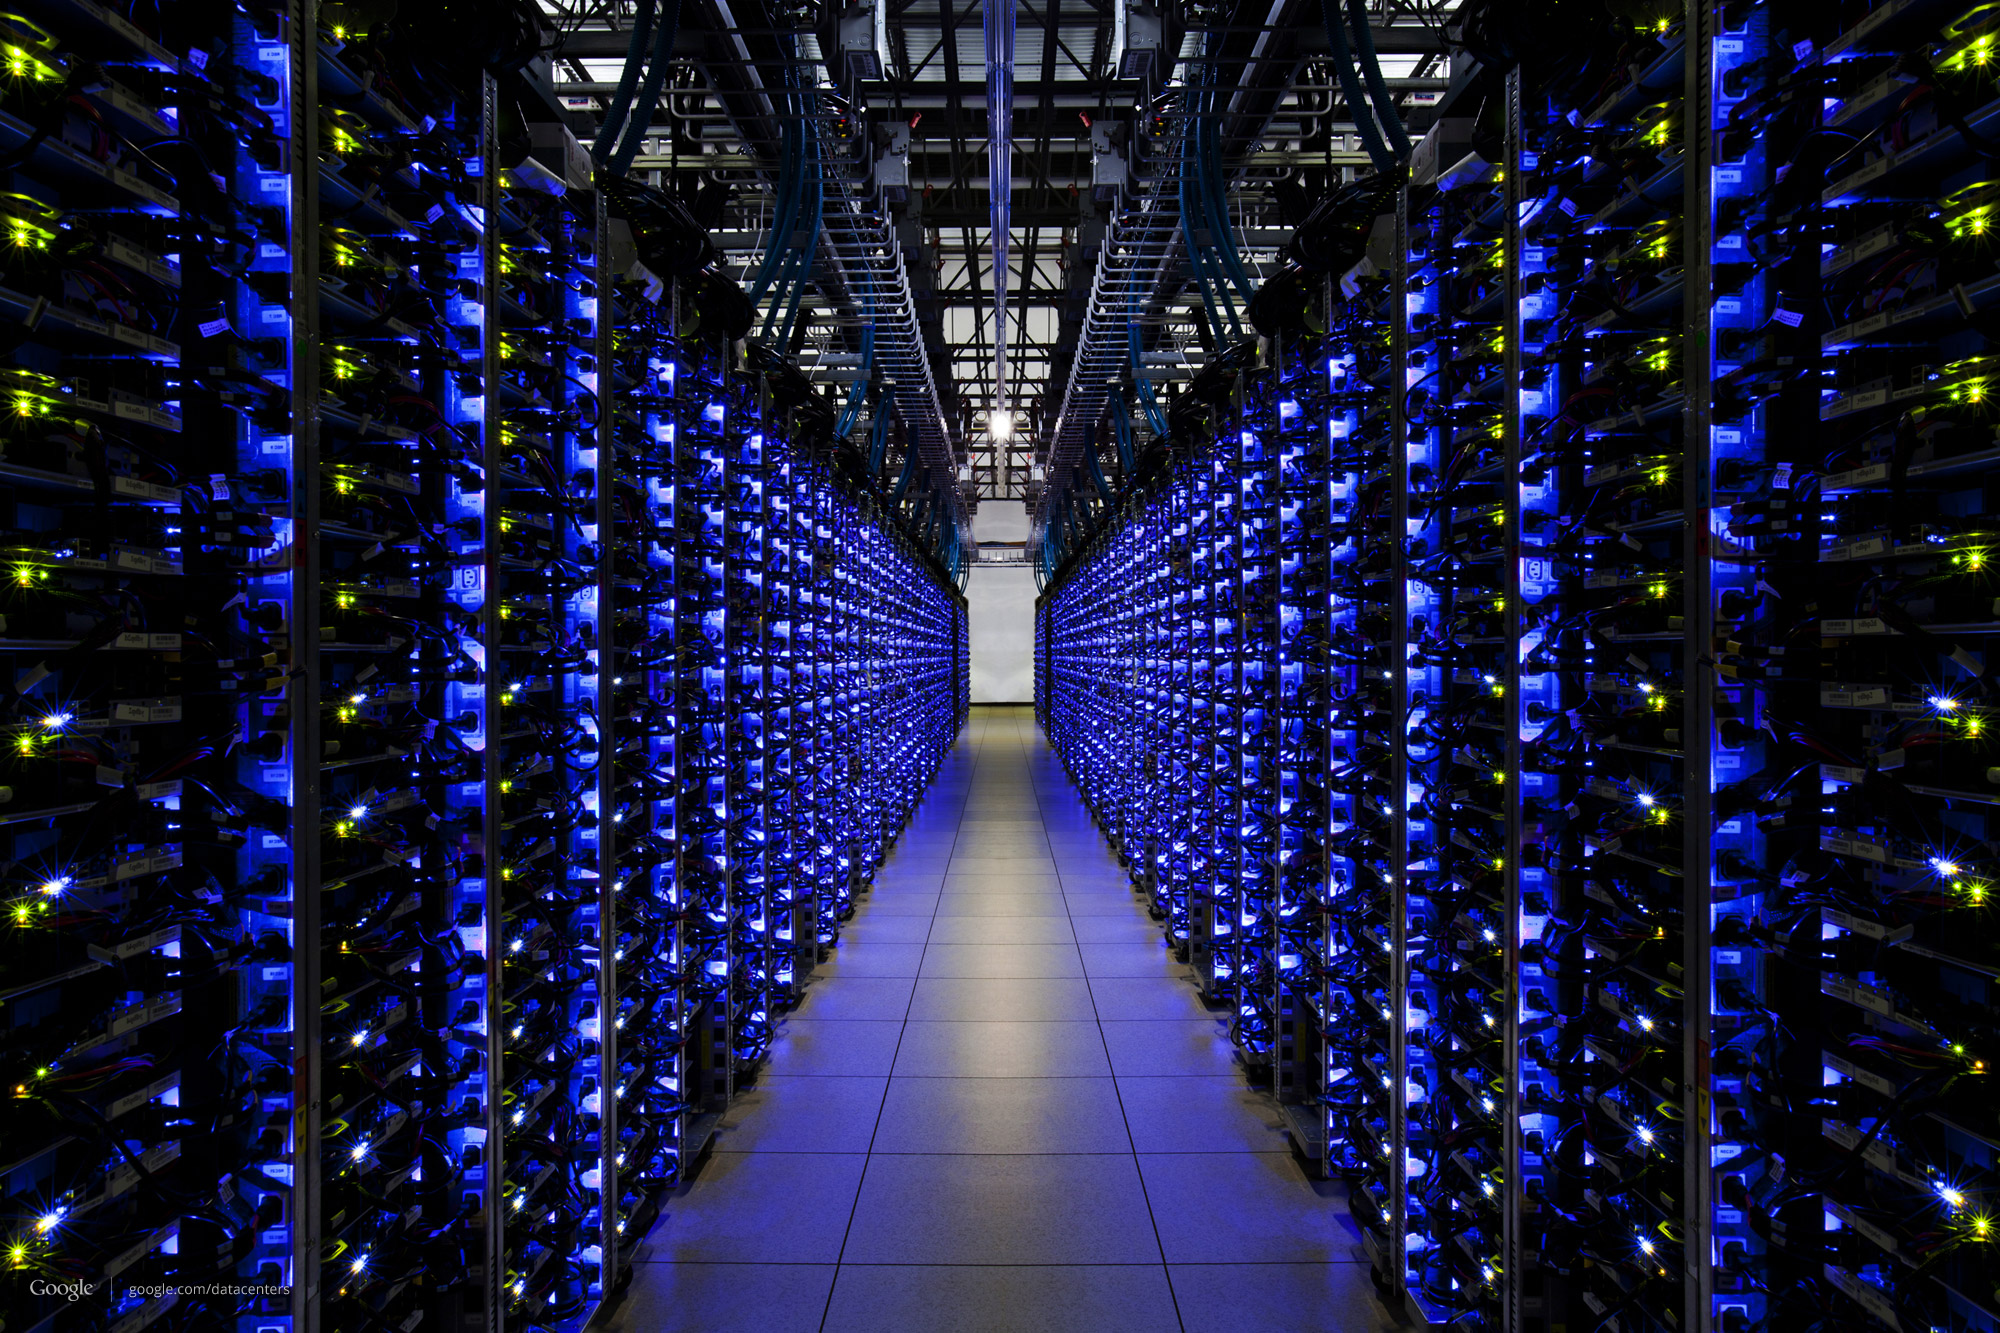
\includegraphics[height=0.5\textheight]{img/data_center.jpg}
\end{frame}
%------------------------------------------------
\section{Model and Problem Formulation}
%------------------------------------------------
\begin{frame}{Model Description}
Input:
\begin{itemize}[<+->]
  \item $m\in\mathbb{N}$\dotso Number of homogeneous servers 
  \item $\beta\in\mathbb{R}_{\ge 0}$\dotso Switching costs of a server
  \item $f:[0,1]\rightarrow\mathbb{R}$\dotso Convex operating cost function of a server
  \item $T\in\mathbb{N}$\dotso Number of time slots
  \item $\lambda_1,\dotsc,\lambda_{T}\in[0,m]$\dotso Arrival rates (workloads)
\end{itemize}
\pause[\thebeamerpauses]
Notation:
\begin{itemize}
	\item $x_1,\dotsc,x_{T}\in\fromto{0}{m}$\dotso Numbers of active servers
\end{itemize}
\end{frame}
%------------------------------------------------
\begin{frame}{Problem Statement}
Operating costs for one time step $t$
\begin{equation*}
	\opcosts(x_t,\lambda_t)\coloneqq\begin{cases}
	  \pause\infty, & \text{if $\lambda_t>x_t$}\hspace{16mm}\text{//too few servers}\\
          \pause 0, & \text{if $x_t=\lambda_t=0$\hspace{9mm}\text{//no active servers}}\\
	  \pause x_tf(\lambda_t/x_t), & \text{otherwise}\hspace{16mm}\text{//even distribution}
	  \end{cases}
\end{equation*}
\pause
\begin{alertbox}
\centering \textbf{Goal: Minimize total costs}
\pause
\begin{align*}
	\text{minimize}\quad \sum\limits_{t=1}^{T}\Bigl(\underbrace{\opcosts(x_t,\lambda_t)+\beta\max\{0,x_t-x_{t-1}\}}_{\costs(x_{t-1},x_t,\lambda_t)}\Bigr)
\end{align*}
\end{alertbox}
\end{frame}
%------------------------------------------------
\section{Optimal Offline Algorithm}
%------------------------------------------------
\begin{frame}{Pseudo-Linear-Time Algorithm}
%\setbeamercovered{invisible}
\centering{Fundamental idea: reduce problem to shortest path problem}
\vspace{-\baselineskip}
\pause \begin{figure}
\resizebox{\textwidth}{!}{
\begin{tikzpicture}[->,>=stealth',auto,node distance=2.2cm,thick,node/.style={minimum size=1.5cm,circle,draw}]
  \node[node] (1) {0,0};\pause
  \node[node] (4) [below right=4cm of 1] {0,1$\downarrow$};
  \node[node] (3) [above =0.5cm of 4] {1,1$\downarrow$};
  \node[node] (2) [above right=4cm of 1] {m,1$\downarrow$};
  \node[node] (5) [below =0.5cm of 2] {m-1,1$\downarrow$};
  \node (22) at ($(2)!.5!(4)$) {};
  \node (23) at ($(2)!.487!(4)$) {\vdots};\pause


  \path[every node/.style={font=\sffamily\small}]
    (1) edge[red] node[black,above left] {$\costs(0,m,\lambda_1)$} (2)
	edge node[label={[xshift=0.8cm, yshift=-0.95cm]$\costs(0,m-1,\lambda_1)$}] {} (5)
	edge node[above right=-0.13cm] {$\costs(0,1,\lambda_1)$} (3)
	edge node[below left] {$\costs(0,0,\lambda_1)$} (4)
    (1) edge ($(1)!.82!(22)$);\pause


  \path[every node/.style={font=\sffamily\small}]
    (2) edge[red] node[black,right] {$0$} (5)
    (3) edge[red] node[black,right] {$0$} (4)
    (5) edge[red] node[black,right] {$0$} ($(5)!.35!(3)$)
    ($(5)!.65!(3)$) edge[red] node[black,right] {$0$} (3);\pause


  \node[node] (7) [right =of 3] {1,1$\uparrow$};
  \node[node] (6) [right =of 2] {m,1$\uparrow$};
  \node[node] (8) [right =of 4] {0,1$\uparrow$};
  \node[node] (9) [right =of 5] {m-1,1$\uparrow$};
  \node (24) at ($(6)!.487!(8)$) {\vdots};\pause

 \path[every node/.style={font=\sffamily\small}]
    (2) edge node[above] {$0$} (6)
    (3) edge node[above] {$0$} (7)
    (4) edge[red] node[black,above] {$0$} (8)
    (5) edge node[above] {$0$} (9);
  \node at ($(23)!.5!(24)$) {\vdots};\pause


  \path[every node/.style={font=\sffamily\small}]
    (9) edge[red] node[black,right] {$\beta$} (6)
    (8) edge[red] node[black,right] {$\beta$} (7)
    ($(7)!.65!(9)$) edge[red] node[black,right] {$\beta$} (9)
    (7) edge[red] node[black,right] {$\beta$} ($(7)!.35!(9)$);\pause


  \node[node] (11) [right =of 7] {1,2$\downarrow$};
  \node[node] (10) [right =of 6] {m,2$\downarrow$};
  \node[node] (12) [right =of 8] {0,2$\downarrow$};
  \node[node] (13) [right =of 9] {m-1,2$\downarrow$};
  \node (25) at ($(10)!.487!(12)$) {\vdots};\pause


  \path[every node/.style={font=\sffamily\small}]
    (6) edge[red] node[black,above] {$\opcosts(m,\lambda_2)$} (10)
    (7) edge node[above] {$\opcosts(1,\lambda_2)$} (11)
    (8) edge node[above] {$\opcosts(0,\lambda_2)$} (12)
    (9) edge node[above] {$\opcosts(m-1,\lambda_2)$} (13);
  \node at ($(24)!.5!(25)$) {\vdots};\pause


  \path[every node/.style={font=\sffamily\small}]
    (13) edge[red] node[black,right] {$0$} ($(13)!.35!(11)$)
    ($(13)!.65!(11)$) edge[red] node[black,right] {$0$} (11)
    (10) edge[red] node[black,right] {$0$} (13)
    (11) edge[red] node[black,right] {$0$} (12);\pause


  \node[node] (15) [right =of 11] {1,2$\uparrow$};
  \node[node] (14) [right =of 10] {m,2$\uparrow$};
  \node[node] (16) [right =of 12] {0,2$\uparrow$};
  \node[node] (17) [right =of 13] {m-1,2$\uparrow$};
  \node (26) at ($(14)!.487!(16)$) {\vdots};\pause


  \path[every node/.style={font=\sffamily\small}]
    (10) edge node[above] {$0$} (14)
    (11) edge node[above] {$0$} (15)
    (12) edge[red] node[black,above] {$0$} (16)
    (13) edge node[above] {$0$} (17);
  \node at ($(25)!.5!(26)$) {\vdots};\pause


  \path[every node/.style={font=\sffamily\small}]
    (17) edge[red] node[black,right] {$\beta$} (14)
    (16) edge[red] node[black,right] {$\beta$} (15)
    ($(15)!.65!(17)$) edge[red] node[black,right] {$\beta$} (17)
    (15) edge[red] node[black,right] {$\beta$} ($(15)!.35!(17)$);\pause


  \node[node] (19) [right =5cm of 15] {1,T$\downarrow$};
  \node[node] (18) [right =5cm of 14] {m,T$\downarrow$};
  \node[node] (20) [right =5cm of 16] {0,T$\downarrow$};
  \node[node] (21) [right =5cm of 17] {m-1,T$\downarrow$};


  \node at ($(18)!.5!(20)$) {\vdots};

  \node (27) at ($(14)!.5!(18)$) {\ldots};
  \node at ($(15)!.5!(19)$) {\ldots};
  \node (28) at ($(16)!.5!(20)$) {\ldots};
  \node at ($(17)!.5!(21)$) {\ldots};
  \node at ($(27)!.5!(28)$) {\ldots};

  \path[every node/.style={font=\sffamily\small}]
    (14) edge[red] node[label={[black,xshift=0cm, yshift=-0.26cm]$\opcosts(m,\lambda_3)$}] {} ($(14)!.4!(18)$)
    (15) edge node[label={[xshift=0cm, yshift=-0.26cm]$\opcosts(1,\lambda_3)$}] {} ($(15)!.4!(19)$)
    (16) edge node[label={[xshift=0cm, yshift=-0.26cm]$\opcosts(0,\lambda_3)$}] {} ($(16)!.4!(20)$)
    (17) edge node[label={[xshift=0.3cm, yshift=-0.26cm]$\opcosts(m-1,\lambda_3)$}] {} ($(17)!.4!(21)$)

    ($(14)!.6!(18)$) edge[red] node[black,above] {$\opcosts(m,\lambda_T)$} (18)
    ($(15)!.6!(19)$) edge node[above] {$\opcosts(1,\lambda_T)$} (19)
    ($(16)!.6!(20)$) edge node[above] {$\opcosts(0,\lambda_T)$} (20)
    ($(17)!.6!(21)$) edge node[label={[xshift=-0.2cm, yshift=-0.26cm]$\opcosts(m-1,\lambda_T)$}] {} (21)

    (18) edge[red] node[black,right] {$0$} (21)
    (19) edge[red] node[black,right] {$0$} (20)
    (21) edge[red] node[black,right] {$0$} ($(21)!.35!(19)$)
    ($(21)!.65!(19)$) edge[red] node[black,right] {$0$} (19);
\end{tikzpicture}}
\end{figure}
\vspace{-0.5\baselineskip}\visible<16-17>{\centering{Time complexity: $\Theta(Tm)$}}

\visible<17>{\ldots only $\log_2(m)$ bits required to encode $m$.}
\end{frame}
%------------------------------------------------
\section{Offline Approximation Algorithm}
%------------------------------------------------
\begin{frame}{2-Optimal Linear-Time Algorithm}
\only<1-2>{\centerline{Use logarithmic steps to reduce number of nodes}
\pause
\begin{figure}
	\includestandalone[width=\textwidth]{../thesis/figures/graph_lin_approx_2}
\end{figure}
\centering where $b\coloneqq\floor{\log_2(m)}$}
\only<3>{\begin{figure}
	\includestandalone[height=0.85\textheight]{figures/schedule_behavior_exmpl}
\end{figure}}
\end{frame}
%------------------------------------------------
\begin{frame}{Approximative Scheduling}
Shortest Path in graph corresponds to 2-optimal schedule.

\pause Time complexity: $\Theta\bigl(T\log_2(m)\bigr)$

\vspace{\baselineskip}
\only<1-2>{\visible<4>{Can we generalize to alllow for arbitrary precisions?}}
\only<3>{\alert{Can we generalize to allow for arbitrary precisions?}}
\only<4>{Can we generalize to allow for arbitrary precisions? \alert{Yes!}}
\only<5>{Can we generalize to allow for arbitrary precisions? Yes!}
\visible<5>{\begin{alertbox} 
\centering Approximation for arbitrary precision $\beps>0$ with time~complexity~$\Theta\bigl(T\log_{1+\beps}(m)\bigr)$
\end{alertbox}}
\end{frame}
%------------------------------------------------
\section{Summary and Prospects}
%------------------------------------------------
\begin{frame}{Summary}
We reduced the scheduling problem to the shortest path problem of acyclic graphs.

\pause
\begin{alertbox}
\centering Optimal Offline Algorithm with pseudo-linear runtime $\Theta(Tm)$
\end{alertbox}
\pause
\begin{alertbox}
\centering $(1+\beps)$-Optimal Offline Algorithm with linear runtime $\Theta\bigl(T\log_{1+\beps}(m)\bigr)$
\end{alertbox}
\end{frame}
%------------------------------------------------
\begin{frame}{Prospects}
Can our approach be modified to\dotso
\pause
\begin{itemize}[<+->]
	\item deal with more than one homogeneous server collection?
	\item deal with multiple sleep states?
	\item work as an online algorithm?
\end{itemize}
\pause[\thebeamerpauses]
Open question: Is there a polynomial optimal algorithm or is it an NP-hard problem?
\end{frame}
%------------------------------------------------
\begin{frame}[standout]
Thanks for your attention!

Any questions?
\end{frame}
%----------------------------------------------------------------------------------------
%------------------------------------------------
\begin{frame}{Data Centers' Costs}
\centering{\Large Fast-growing demand for data collection, processing, and storage}

\vspace{0.5\baselineskip}
\centering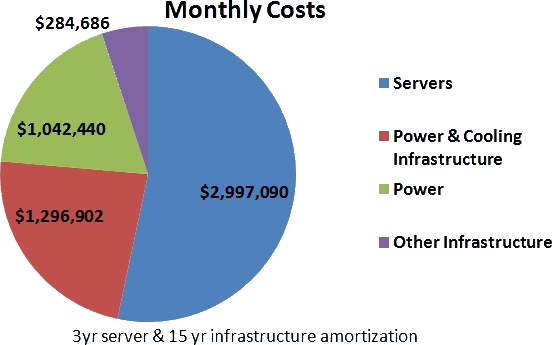
\includegraphics[height=0.5\textheight]{img/data_center_costs.jpg}
\end{frame}
%------------------------------------------------
\begin{frame}{Proof Idea}
\centering Take a schedule and transform periods between two powers of 2

\pause\begin{figure}
	\includestandalone[width=0.85\textwidth]{figures/schedule_behavior}
\end{figure}
\end{frame}
%------------------------------------------------
\begin{frame}{$(1+\beps)$-Optimal Offline Algorithm}
\begin{figure}
	\includestandalone[width=\textwidth]{../thesis/figures/graph_lin_approx_y}
\end{figure}
\centering where $y\coloneqq1+\beps,b\coloneqq\floor{\log_y(m)}$
\end{frame}
%------------------------------------------------
\begin{frame}[allowframebreaks]{Image Sources}
\begin{itemize}
\item Data center: \url{datacentervoice.com/wp-content/uploads/2015/12/data-center.jpg}
\item Data center costs: \url{perspectives.mvdirona.com/2008/11/cost-of-power-in-large-scale-data-centers/}
\end{itemize}
\end{frame}

\end{document} 
